\documentclass[a4paper,11pt]{article}
\usepackage[margin=2cm]{geometry}

\usepackage[titletoc,toc,title,page]{appendix}
\usepackage[nodayofweek]{datetime}
\usepackage{cite}
\usepackage{graphicx}
\longdate



\usepackage{paralist}
\usepackage{mathcomp}
\usepackage{bm}
\usepackage{amsmath,amssymb,amsthm,enumitem}
\usepackage{graphicx}
\usepackage{caption}
\usepackage{subcaption}
\usepackage{titlesec}

\setcounter{secnumdepth}{4}

\usepackage{hyperref}
\usepackage{fancyhdr}
\usepackage{minted}
\pagestyle{fancyplain}
\fancyhf{}
\lhead{\fancyplain{}{M.Sc.\ Group Project Report}}
\rhead{\fancyplain{}{\today}}
\cfoot{\fancyplain{}{\thepage}}

\usepackage{minted}







\title{Implementation of attentional bistability of the dragonfly visual neurons in an intelligent biomimetic agent\\\Large{--- Final Report ---}}
\author{Juan Carlos Farah, Panagiotis Almpouras, Ioannis Kasidakis, Erik Grabljevec, Christos Kaplanis\\
       \{jcf214, pa512, ik311, eg1114, ck2714\}@doc.ic.ac.uk\\ \\
       \small{Supervisors: Professor Murray Shanahan, Zafeirios Fountas, Pedro Mediano}\\
       \small{Course: CO530/533, Imperial College London}
}

\begin{document}
\maketitle

\tableofcontents

\clearpage
\section{Introduction}

Dragonflies are insects of the order Odonata, suborder Anisoptera \cite{dfwiki}. They are notoriously effective at prey capture, with success rates ranging from 76\% to 97\% \cite{Olberg2011}, making the neural processes that underlie this ability particularly interesting to investigate. There has been substantial research into the visual system of dragonflies \cite{Wiederman2008, w13} but what seems to be lacking is an effective tool that links models of the various mechanisms involved in this process together, which could help us better understand the particular function of each layer within the system.

At the core of this apparatus, the centrifugal small target motion detector one neuron (CSTMD1) is a higher order visual neuron in the brain of the dragonfly that reacts to the presentation of multiple visual stimuli by firing as if only one of the stimuli was present. This is presumably an attentional selection mechanism \cite{w13}. At Professor Murray Shanahan's lab, researchers have simulated the large contralateral dendritic field of the CSTMD1 neuron with a biophysical multi-compartmental Hodgkin-Huxley model. Along with Klaus Stiefel \cite{ne13}, they found that with certain numbers of inhibitory synapses and potassium conductance densities, two mutually-coupled CSTMD1 neurons are capable of a bistable switching process between two input patterns. In order to confirm that this neuron is indeed responsible for target selection, it would be useful to be able to model the CSTMD1 as a part of a whole visual system. Our goal was to create a tool that could hopefully serve the following purposes:
\begin{enumerate}
\item Provide a connected model of dragonfly target selection, starting from the visual input to the retina and ending with the motion of the dragonfly.
\item Provide a graphical interface for each module and for the system as a whole, allowing users to run simulations and view useful information on the processing done by each layer.
\item Provide persistent, easily accessible storage of experimental data generated by the individual layers and the system as a whole.
\item Provide a platform for potentially replicating the behaviour of a real dragonfly during prey capture.
\end{enumerate}

\subsection{Report Structure}
The parts that this report includes are the following:\\

\noindent
\textbf{Specification:}
This section outlines our original goals and how they were adjusted according to the challenges that were encountered during development. We also present the motivation behind additional goals that were set to ensure a balanced workload and to achieve the best possible results given the high level of complexity and the time constraints of the project.\\

\noindent
\textbf{Design:} This section provides an overview of the design for our project. Particular attention is given to the options that were considered and the justification of the choices made for each component individually and for the system as a whole.\\

\noindent
\textbf{Methodology:} This section highlights the specific techniques, frameworks and solutions used to meet the goals set forth in the specification. We present the problems and challenges that were faced during the project and explain how we tackled them, with the architecture and implementation of each module being considered in detail. Additionally, we explain our software development strategy and how it helped us address those issues effectively.\\

\noindent
\textbf{Group Work:} This section illustrates how we divided our project into small, measurable tasks. We also describe how we divided into sub-groups that could develop each module in parallel and how this allowed us to maximise our throughput given the time constraints.\\

\noindent
\textbf{Final Product:} This section present the final product of the work conducted throughout the project, expanding on the goals that were met as well as the goals that were infeasible. We analyse results in detail and motivate future development as well as potential extensions that might be of interest to future collaborators.\\

\noindent
\textbf{Appendix:} This section presents a log of the summary of the minutes for meetings conducted throughout the project, covering tasks assigned to each member and his overall contribution. 

\section{Specification}

Our initial approach to establishing the requirements for this project was to brainstorm using goal-oriented capture. As depicted in Figure 1, our initial goal was to create a biomimetic agent that emulates target selection in the dragonfly. 
	
	\begin{figure}[h]
	\begin{center}
	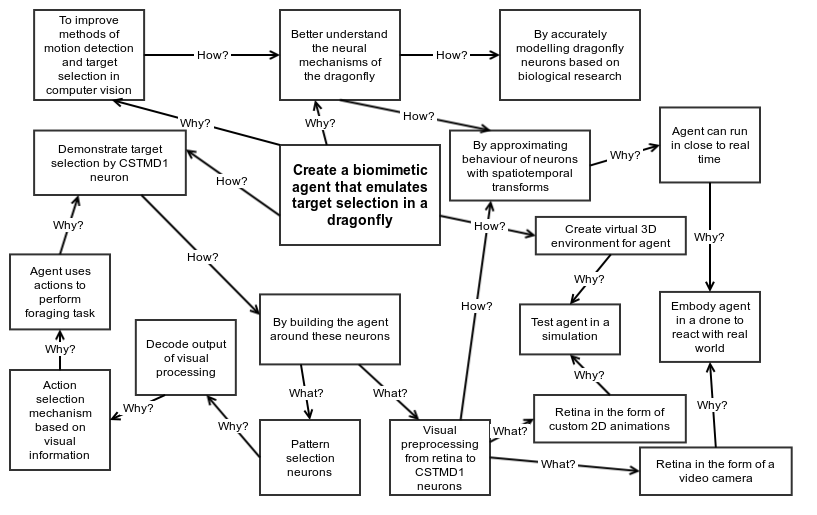
\includegraphics[scale = 0.5]{goalorient}
	\end{center}
	\caption{Goal-Oriented Capture Diagram}
	\end{figure}	
	
	Goal-oriented capture enabled us to identify the minimum requirements for the completion of our project. As we progressed in the development of the system, we ran into some complications that motivated us to modify the certain aspects of our specification. 
\subsection{Challenges and Motivation for Updated Specifications}
In this section, there is a brief discussion of the challenges that were faced during the project and how they motivated the adjustment of the original specifications.

	At the start of the project, our main objective was to create a working dragonfly target selection system. Key to the implementation of a biomimetic agent was the functioning of the CSTMD1 neuron, which had been previously modelled at Professor Shanahan's lab. Having previously displayed evidence of bistability, it was expected that the model of the CSTMD1 would be capable of selecting one target from many in the dragonfly's visual field by replicating the results of research done into real CSTMD1 neurons \cite{w13}. Despite the hard work that was put into addressing the issue, the complex morphology of the CSTMD1 neuron made the task infeasible to be fully completed within the time frame of this project. Thus, it was moved to possible extensions and although significant progress was observed, it was only partially completed by the submission deadline.
	
	Furthermore, our difficulties led us to believe that it would be useful for us and for future researchers into dragonfly vision to create a user-friendly interface for interacting with our dragonfly system. To this end, we decided to add the creation of a web client to our requirements. The aim is for the web client to provide an interface that allows the user to run and save simulations of either each module individually or of the whole system and to provide key metrics that demonstrate the functionality of each part.
	
\subsection{Final Specifications}
The following table summarises the finalised requirements and the level of completion for each part.
\begin{center}
    \begin{tabular}{p{12cm} c c}
    \textbf{Minimum Requirements (Stage 1)} & \textbf{Completion} \\ \hline
    (Ai) Create an animation tool to generate inputs for visual processing. & Full \\ 
	(Aii) Build a model for the ESTMD neuron present between the retina and the actual CSTMD1 neurons of a real dragonfly. & Full \\
	(Aiii) Design connection between ESTMD and CSTMD1 neurons. & Full \\
	(B) Build a layer of pattern recognition neurons that can learn to recognise spike patterns within a noisy background. & Full\\
	(C) Integrate the visual processing and pattern recognition system to detect patterns within the CSTMD1 output and add a simple action selection mechanism. & Full\\
    \end{tabular}
\end{center}

\begin{center}
    \begin{tabular}{p{12cm} c c}
    \textbf{Expected Implementation (Stage 2)} & \textbf{Completion} \\ \hline
	(A) Develop a web client to analyse metrics of each component in our model. & Full \\
	(B) Create an animation for the dragonfly agent. & Full\\
	(C) Enhance the action selection mechanism to control the agent within the environment. & Full\\
    \end{tabular}
\end{center}

\begin{center}
    \begin{tabular}{p{12cm} c c}
    \textbf{Possible Extensions (Stage 3)} & \textbf{Completion} \\ \hline
	(A) Improve the usability and features of the web client. & Full\\
	(B) Achieve CSTMD1 target selection through experimentation with various parameters and connections with the ESTMD neurons. & Partial\\
	(C) Implement the agent in a quadcopter drone. & None\\
    \end{tabular}
\end{center}






\clearpage
\section{Design}

The challenge of designing a tool that could satisfy the overall functionality outlined in the introduction could be distilled down to two main facets:
\begin{enumerate}
\item Deciding on the components of the dragonfly visual system and how they would be connected together.
\item Deciding on the user interface and specifying an API for the system.
\end{enumerate}

\subsection{System Components}

Building on research done at Professor Murray Shanahan's laboratory on the CSTMD1 neuron \cite{?}, our first design challenge was to specify the structure of the system that we would build around the CSTMD1. We identified four key components that we would need to model and connect in order to implement a coherent system. Along with the CSTMD1, they make up the main modules in our project.

\begin{enumerate}
\item \textbf{Target Animation:} This module's purpose is to provide sample ``prey'' that our biomimetic agent can identify and ``capture''. Our implementation allows the user to specify movements of multiple targets within the visual field and choose the background, resulting in an animated video that provides the visual input to the system. Biologically this emulates the retina of the dragonfly.

\item \textbf{Elementary Small Target Motion Detector (ESTMD):} The ESTMD neurons are the first layer of visual processing in the dragonfly. They have the general function of identifying and isolating small moving targets, even against a cluttered, moving background \cite{Wiederman2008}. They take arrays of pixel values as input from the animation and output firing rates of neurons to be processed by the next layer.

\item \textbf{Centrifugal Small Target Motion Detector One (CSTMD1):} The CSTMD1 neuron is a higher order visual neuron in the brain of the dragonfly. This neuron reacts to the presentation of multiple visual stimuli by firing as if only one of the stimuli was present \cite{w13}. The CSTMD1 takes the firing rates of the ESTMD as input and outputs a time series of neuron spikes (spike trains) to the next layer.

\item \textbf{Pattern Recognition:} This module has the function of detecting patterns in the output of the CSTMD1 in order to distil features of target movement within the visual field. While it does not have a direct correspondence to a layer of neurons in the dragonfly, it uses a well-established biological learning mechanism called Spike Timing Dependent Plasticity (STDP), which we discuss in section X.X.X. Its purpose is to encode information in the CSTMD1 output and pass it onto the Action Selection module.

\item \textbf{Action Selection:} This module takes as input the spike trains from the pattern recognition neurons and the original target animation video. Its function is to select an action for the biomimetic agent at each time step given that input. Biologically, our model emulates the connection between the visual processing and the motor neurons. It can be trained using STDP combined with reward modulation so that the dragonfly learns to maximise target capture based on recurring patterns in its visual field. The final output is the original animation with the position of the dragonfly superimposed onto each frame for observation of how effectively it chases targets.
\end{enumerate}

\subsection{User Interface}
As we developed the aforementioned modules, we recognised the need to provide an user-friendly interface to our system. In order to maximise portability, the solution had to be lightweight and cross-platform. The most suitable architecture for this purpose consisted of a framework that could connect to each of our modules and provide a client that could be run any modern browser.

Our web client is designed to be a simple interface that allows for simulations for each of the modules to be run and automated, either separately or jointly. This graphical user interface interacts with each module's API and provides the functionality needed to save and access the results of every experiment. It also provides key metrics that can be crucial in understanding the performance of the system.

\subsection{Data Store}

Given the computationally expensive nature of our modules' simulations, a persistent store had to be used to save the output and results of each run. As shown in the structure diagram below, the five modules that our project comprises, are connected sequentially. Saving the output of each module enabled us to reuse the output of a module as input to the next, multiple times without the need to rerun any of the previous modules. Furthermore, the persistent store allows the web client to provide a view of the results for analysis simply by querying the database instead of regenerating them each time.

For our data store MongoDB \cite{mdb} was chosen. MongoDB provides a fast, scalable solution that does not require strict design decisions in advance. Considering in retrospect the changes and adaptations that had to take place during this project, we trust that MongoDB was a wise choice that contributed to the overall success of this project.


\subsection{Design diagram}
The following figure provides a graphical representation of the system as whole. 

\begin{figure}[h]
\centering
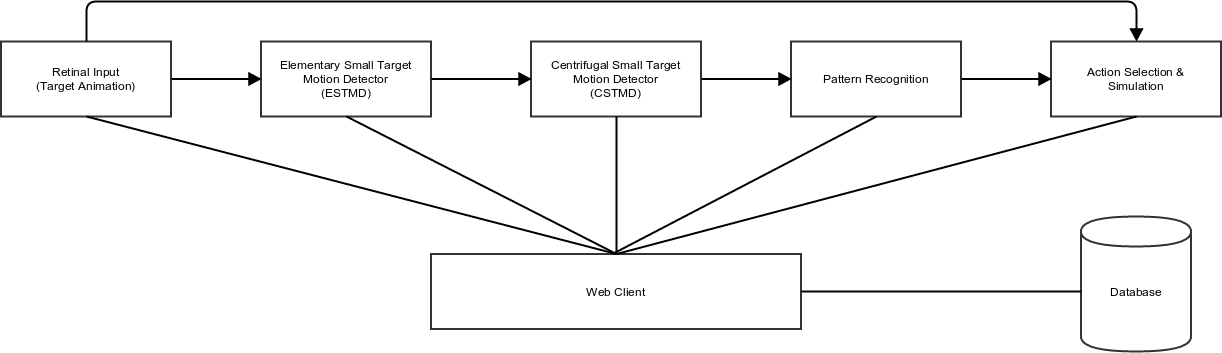
\includegraphics[scale = 0.35]{designblockdiagram2}
\caption{Project Structure Diagram.}
\end{figure}

\subsection{Programming language}
In order to maintain consistency throughout the project, all modules were programmed in the same language. This facilitated communication between the modules as well as their respective link to the web client. Additionally, it allowed us to run one test suite that comprehensively covered the whole project. We decided to use Python \cite{python} for this project given our team's experience with the language as well as its flexibility and ubiquity. Python includes libraries for efficient matrix manipulations that were key in most of the modules, as well as a vast number of neuroscience-specific modules that allowed us to develop our project without having to write potentially complex low-level functions. Furthermore, Python's matplotlib 2D plotting library provides a way for each module to generate production quality graphics that can be easily transmitted to an interactive user interface.


\clearpage
\section{Methodology}
Having decided upon a number of specific modules required for the biomimetic agent, the project was naturally split into subproblems in the form of these modules. Additionally, the sequential nature of the modules within the system meant that it made sense to start by building the input of the system first and progress towards the final output, so that the connections between modules could be tested along the way. The web client was built in the latter stage of the project as it was most important to make sure the components of the system worked before building the user interface. Below, we describe the detailed methods undertaken in completing each module, as well as an overview of the software engineering techniques we used, our testing methodology and summary of the coverage achieved by our test suite.

\subsection{Target Animation}
This module represents the input to the dragonfly's retina. Our goal was to create an animation tool that would allow a user to flexibly create videos of moving targets against a custom and potentially moving background. Our initial specifications aimed to create a 3D animation, where the dragonfly's view would change dynamically depending on the dragonfly's position and orientation. As a first step, we implemented a 2D animation, with coloured circles representing targets against a moving or stationary background that could be defined by the user.

The design of this module was approached from the user's perspective. Our priorities were to provide flexibility through a simple interface through which to define the duration and size of the video, specify a background, and add targets, each with potentially different properties and behaviours. We supported two types of targets, the first displaying random movement across the viewport and the second moving in a straight line. For the former, the user could simply specify the starting position and speed. For the latter, the user was required to set the target's direction of travel. Additionally, the background could be provided as a PNG or JPG file and would be automatically cropped to fit the viewport.

\begin{figure}[ht]
\centering
\begin{minipage}{0.2\textwidth}
\fbox{
\includegraphics[scale = 0.14]{ran0}}
\end{minipage}
\begin{minipage}{0.2\textwidth}
\fbox{
\includegraphics[scale = 0.14]{ran1}}
\end{minipage}
\begin{minipage}{0.2\textwidth}
\fbox{
\includegraphics[scale = 0.14]{ran2}}
\end{minipage}
\begin{minipage}{0.2\textwidth}
\fbox{
\includegraphics[scale = 0.14]{ran3}}
\end{minipage}
\caption{Simple example of Target Animation output. The black dot represents the target.}
\label{target_animation_example}
\end{figure}

\begin{figure}[h]
\centering
\begin{minipage}{0.2\textwidth}
\fbox{
\includegraphics[scale = 0.14]{str0}}
\end{minipage}
\begin{minipage}{0.2\textwidth}
\fbox{
\includegraphics[scale = 0.14]{str1}}
\end{minipage}
\begin{minipage}{0.2\textwidth}
\fbox{
\includegraphics[scale = 0.14]{str2}}
\end{minipage}
\begin{minipage}{0.2\textwidth}
\fbox{
\includegraphics[scale = 0.14]{str3}}
\end{minipage}
\caption{Simple example of action selection output. The red dot represents the dragonfly focal point and the black dot represents the target.}
\label{target_animation_example}
\end{figure}

The challenge was to turn this information into an animation. Our approach was to first create a sequence of images given the input from the user which could then be sequenced into a video. We decided to build our implementation using Gizeh \cite{gizeh}, a Python library for vector graphics written on top of cairocffi \cite{cairocffi} the Python binding for Cairo \cite{cairo}, a 2D graphics library written in C. Gizeh allowed us to perform image creation and manipulation efficiently, as it offers function calls for some of our key requirements, such as drawing circles, adding background images, scaling and transforming graphics. Hence the core of the target animation module processes the user-generated input, calculates the position of each target and of background at each frame and computes the location where each target should be drawn and how the background image should be rendered. At each step, we save the generated image to a temporary file. The generated sequence of images is then combined into a video using OpenCV \cite{opencv}, an an open source computer vision library, and exported as an AVI file. Additionally, the module outputs the series of images in matrix format consisting of greyscale pixel values, which are passed as input to the ESTMD module, and converts the AVI file MP4 format so that it can be easily rendered in a browser using HTML5.
\newline
\newline
Example of frame in produced video can be seen on the picture  ~\ref{target_animation_example}.

\begin{figure}[h]
\centering

\includegraphics[scale = 0.3]{ta}
\caption{Simple example of action selection output. The red dot represents the dragonfly focal point and the black dot represents the target.}
\label{target_animation_example}
\end{figure}


The target animation module is also required to produce the final output of the visual system, where the biomimetic agent is shown ``chasing'' the targets from the initial input video. Rather than create a whole new animation where the whole dragonfly is visible, we decided to superimpose the dragonfly's visual focal point as a distinctive circle on the original animation. This means that the ``chasing'' is represented as the point in the visual field that the biomimetic agent is focusing on. In order to assist with the reward-modulated learning provided by the action selection module, the target animation module exposes functions to calculate positions of targets at any given time during the animation. This allows the action selection module to appropriately implement reinforcement learning and is further discussed in section X.X.

\subsection{Elementary Small Target Motion Detector (ESTMD)}

In our initial specification, one of our tasks was to connect the retina of our dragonfly to the CSTMD neurons. Having researched how this occurs in real dragonflies, we discovered that we would have to include a layer of neurons that preprocesses the input from the retina before passing it on to the CSTMDs, named elementary small target motion detectors (ESTMD) \cite{Wiederman2008}. While one of the purposes of the CSTMD seems to be to give the ability to select one target among many in the visual field \cite{w13}, the function of the ESTMDs seems to be that of identifying small moving targets, even against a cluttered, moving background \cite{Wiederman2008}.
\newline
\newline
Our research revealed that the ESTMDs actually consist of several layers of neurons required to perform their function, namely photoreceptors, large monopolar cells (LMCs) and rectifying transient cells (RTCs) \cite{Wiederman2008}. It was immediately obvious to us that implementing all these stages in a multi-compartmental model (the method used for the CSTMD) would be extremely complicated and computationally expensive. Our initial thought was to attempt to use simplified point neuron models (such as Integrate-and-fire) to achieve the ESTMD function, but with a little more research we discovered that it would be possible to do it in a simpler and more computationally efficient way using a series of spatial and temporal transforms on the retina input \cite{Wiederman2008} \cite{hal11}. It is important to note that these transforms are intended to directly approximate the layers of biological neurons mentioned above - there are other techniques from computer vision that could be used for small target motion detection, but our priority is to represent the true function of the dragonfly's brain within realistic bounds of computational complexity. The overview of the model we implemented is summarised in Figure 1 and the details of the transforms were taken from \cite{hal11}. 

\begin{figure}[h]
\centering
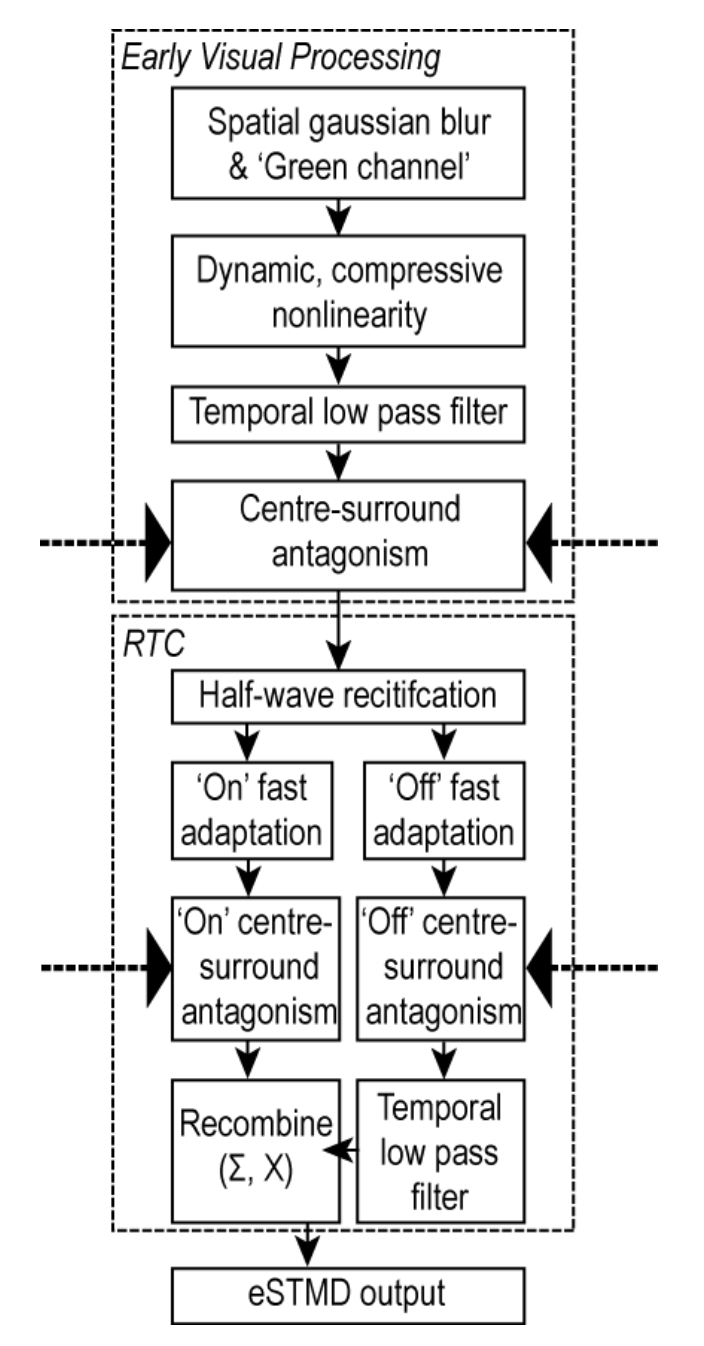
\includegraphics[scale = 0.5]{wiederman09}
\caption{\cite{Wiederman2008}}
\end{figure}

The first consideration we had to take was the input and output of the ESTMD module. The input would be a time series of two-dimensional arrays of pixel values from the retina and the output would need to be a time series of neuron spikes (spike trains) to provide input to the CSTMD. The spatial and temporal transforms we intended to use are directly applicable to an array of pixel values but the output of these transforms would also be an array of pixel values that would need to be transformed into spike trains. We decided the simplest and most efficient way of doing this would be to map each pixel value to a corresponding firing rate of a neuron, but this would be dealt with by the CSTMD module. In addition, to demonstrate the effect of the ESTMD module, we decided that it would be useful to provide a video of the output in order to ascertain visually that it is performing its expected function.
\newline
\newline
One significant challenge was understanding the transforms and implementing them in Python. For example, understanding the transforms required some background reading on z-transforms, which are the discrete equivalent of Laplace transforms, which are necessary as our system works in discrete time steps. For the translation of the model into Python, we used the Scipy.signal and openCV \cite{opencv} libraries extensively: Scipy was used to process the z-transforms (the temporal transformations) and openCV was used for the spatial transforms, such as Gaussian filtering. We also used openCV to convert videos into arrays of pixel values and vice versa.
\begin{figure}[h]

\includegraphics[scale = 0.4]{input}

\includegraphics[scale = 0.5]{processed}
\caption{Snapshot of target animation and example of the corresponding ESTMD output. The target is circled in red in the original animation.}
\end{figure}

Once we had programmed the transforms, some tinkering with parameters was required to achieve the small target motion detection we were expecting. In any case, the user of the web client will have the capability of changing these parameters for their own model.

\subsection{Centrifugal Small Target Motion Detector Neuron (CSTMD)}

The function of this module is to implement a multi-compartmental model of the actual CSTMD neuron that exists in dragonflies, with the hope that it will create an effect of selecting one target from many in the visual field. It takes input from the ESTMD and gives output to the pattern recognition module. The initial code was given to us by our supervisors, who had already shown that there is mutual inhibition of CSTMD1 neurons that could indicate target selection, but it was our job to connect it to the rest of the system and also, as a secondary goal, see if we could replicate the target selection effect observed in real dragonflies. The main issues in tackling this model were:
\begin{enumerate}
	\item Understanding he complicated nature of the morphologically-modelled CSTMD1
	\item Learning how to use the simulation environment of the CSTMD1 neurons (NEURON simulation environment)\cite{neuron}
	\item Efficiently connecting this module with both the ESTMD and the pattern recognition module
	\item Generating key indicators to measure the performance and the plausibility of the module, in order to assist the user in assessing the function of this neuron
\end{enumerate}

Given that the CSTMD1 is multi-compartmental model with several parameters that directly or indirectly affect its activity and effect to a given input, we needed to first fully understand the given model before proceeding with any further decisions. Thus, we performed several tests in order to be aware of all the plausible values that should be tried for each of the parameters.

Moreover, we had to consider what would be the best way to provide stimuli to the CSTMD1 neurons as an input from the ESTMD module. The NEURON simulation environment provides many classes as a connection to a model from an external input. After examining all the different possibilities we decided to use a leaky integrator (IntFire2() point process). We made this selection as it allows the modification of the total current as a parameter which is what we required in order to connect the two modules. IntFire2() also has a quite straightforward structure compared to other similar but considerably more complex point processes. 

The ESTMD module provides a time series of neuron spikes which is essentially an array of values each of which corresponds to a spiking rate per retina pixel. Thus, we initiated one leaky integrator for each pixel and provided the spiking rate as its total current. We then connected these point processes to each of the CSTMD neurons used for the simulation. In order to make our model as much biologically plausible as possible, we added some randomized delays to the connections of the leaky integrators with the CSTMD1 neurons with the aim of ensuring that the desired inhibitory effect will be achieved while neurons are provided with some stimuli. We also applied a spatial Gaussian distribution to the weights of these connections, increasing the relative weights of the pixels in the centre of the visual field compared to those on the edges, as this is the case with real dragonflies \cite{w13}.

With regards to the output, since the pattern recognition module requires a considerable number of spike trains as an input, we had to find a way to connect the 2 modules without severely affecting the speed and performance of the CSTMD1 module. Hence, given the morphologically large axon of the CSTMD1 neuron \cite{geurten} we decided that, instead of using as many neurons as the inputs required by the pattern recognition module, to apply a large number of electrodes to different compartments of the neurons and thus provide the adequate number of spike trains without limiting the biological plausibility of our model.

After successfully connecting the different modules, our next goal was to define key performance indicators for the CSTMD1 module in order to measure as accurately as possible its performance and also be able to modify the several parameters of the given model and observe their effect to the simulation. For this purpose, we created several plots which recorded the activity of different compartments of the neurons as well as their spiking rates. 


\begin{figure}[h]
\centering
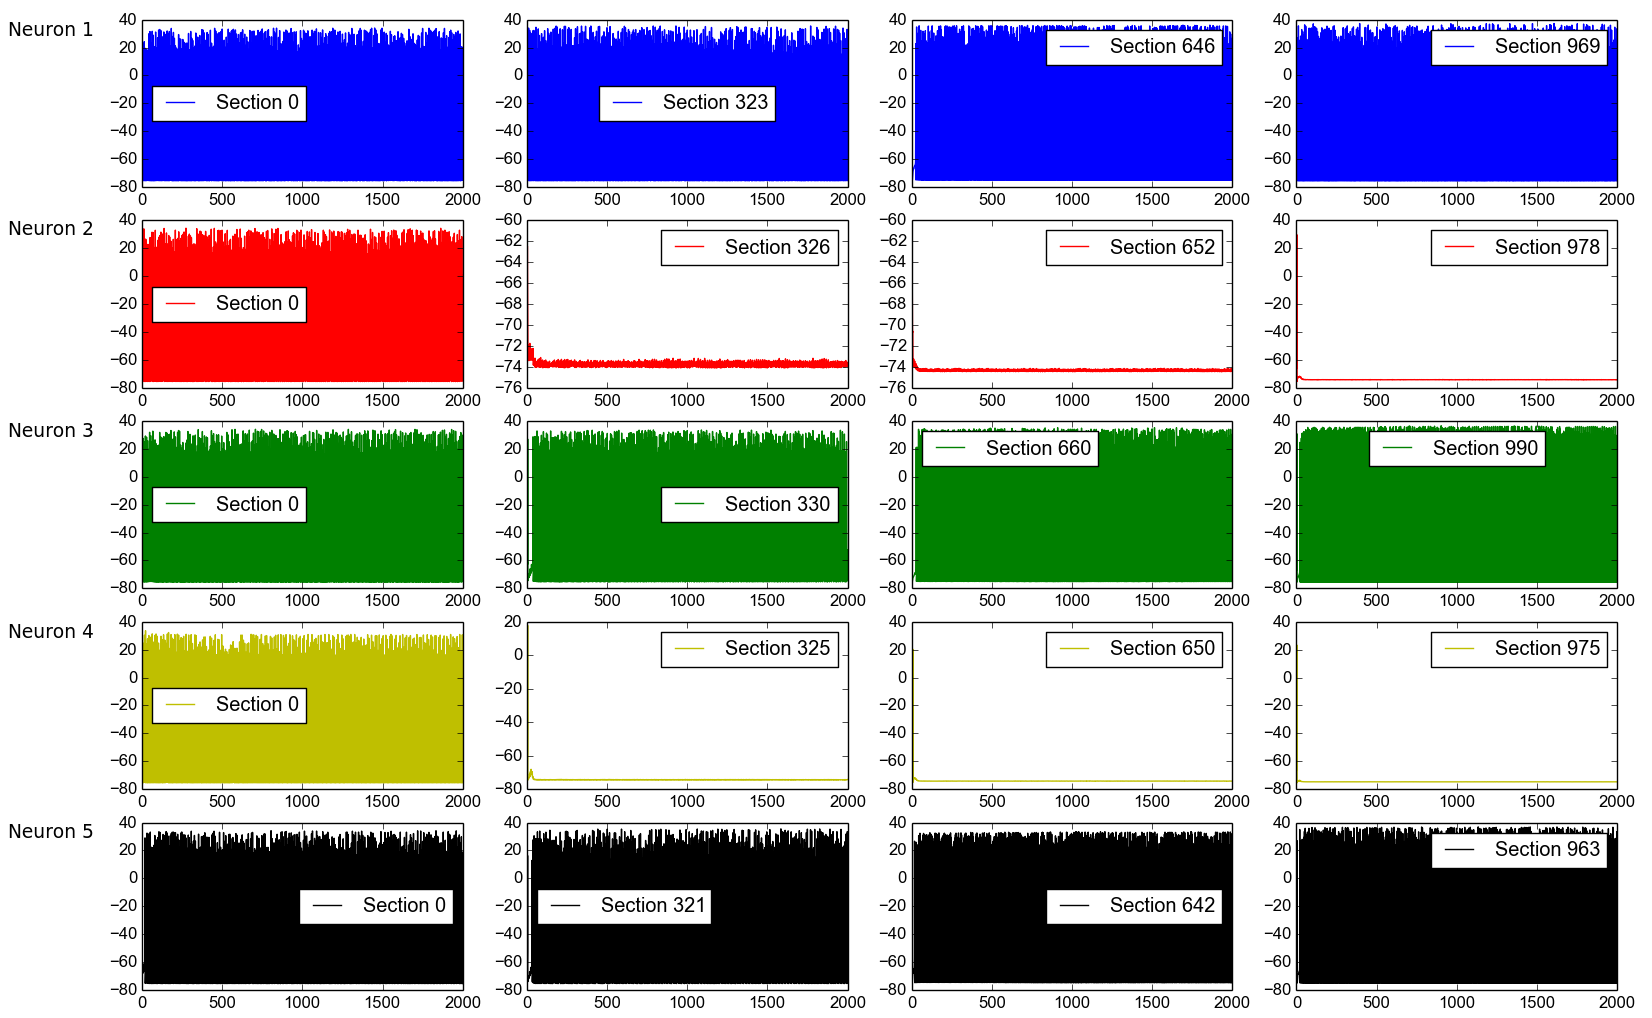
\includegraphics[scale = 0.3]{compartments}
\caption{Compartmental activity in a CSTMD1 neuron simulation showing inhibitory effects}
\end{figure}

The above figure shows the spiking rate of different compartments of 5 CSTMD1 neurons as these were used in one of our simulations in the NEURON simulation environment. We can observe that most compartments of the 2nd and the 4th neuron, coloured in red and yellow respectively, show little or no spiking activity although they seemed to have received similar stimuli to their counterpart neurons as shown by the spiking rates of their initial compartments in section 0. Hence, an inhibitory effect is evident which results in neurons 1, 3 and 5 having high spike rates whereas neurons 2 and 4 show a blockade of activity.

We also extended the module to be able to run several simulations while given different inputs from the ESTMD module so as to observe if there is any evidence that our CSTMD1 module, when presented with two targets in the visual receptive field, would select one of them as we expected. However, after modifying all the possible parameters and trying different inputs, we observed that the CSTMD1 model is not displaying this selectivity.

\begin{figure}[h]
\centering
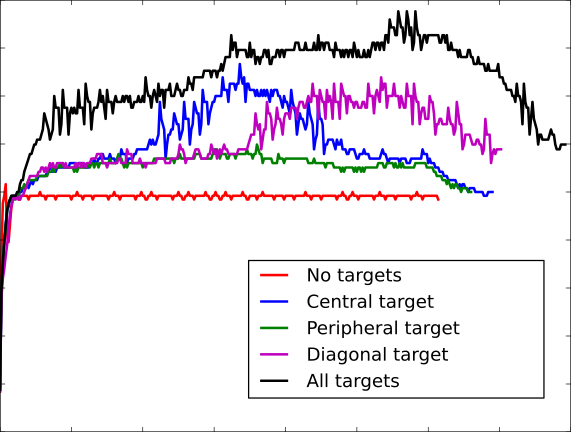
\includegraphics[scale = 0.5]{3targets}
\caption{Firing rates of CSTMD1 neurons given varius inputs}
\end{figure}

As shown in the above figure, we performed 5 different simulations in order to come to this result. We tried running the CSTMD1 simulation while giving different stimuli and we recorded their spiking rates. The lowest spiking activity is the one which corresponds to the simulation where no targets were presented. The blue, purple and green lines show variable spiking rates and correspond to simulations were targets in different positions were presented(central target, diagonal target and peripheral target respectively). However, when we performed a simulation where all targets were presented, the CSTMD1 neurons did not show any selectivity by resembling the spiking activity to the ones in the previous simulations and thus we were not able to replicate the results of \cite{w13}.Instead, what we are observing is a CSTMD1 neuron that fires more frequently when all targets are present.

The web client that we introduced supports running simulations of the CSTMD1 module. We transferred all the functionality as described above and thus the user is able to change all the significant parameters of the model and observe the resulting CSTMD1 neurons' behaviour as well as the behaviour of KPIs in the model.

\subsection{Pattern Recognition}

The purpose of the pattern recognition module is to discern recurring spike patterns within the output from the CSTMD1 module, with each pattern recognition neuron becoming selective to one pattern. Given the expected behaviour of CSTMD1 neurons, as explained in Section XX, we hypothesised that any patterns found in the output of the CSTMD1 module would encode information about the velocity and direction of targets observed in the visual field of the dragonfly.\par

	In order to model these neurons, we initially replicated experiments conducted by Masquelier et al. \cite{stdp2} \cite{stdp1}. These experiments showed that spike response model (SRM) leaky integrate-and-fire (LIF) neurons could successfully recognise input patterns based on sample input generated from a Poisson process. A single neuron of this type is able to successfully recognise a recurring pattern within background noise and a network of them is able to do so for multiple patterns. This behaviour is achieved by modulating the weights of the pattern recognition neuron's synaptic connections to its afferents using spike timing dependent plasticity (STDP). STDP uses Long Term synaptic Potentiation (LTP) to reinforce connections with afferents that fired shortly before the postsynaptic neuron, and Long Term Depression (LTD) to weaken those with afferents that fired shortly after. Given that the input patterns occur within random noise, STDP will favour those afferents that participate in the pattern, as every time the pattern manifests itself, they will consistently fire in a given order.
	
\begin{figure}[H]
\centering
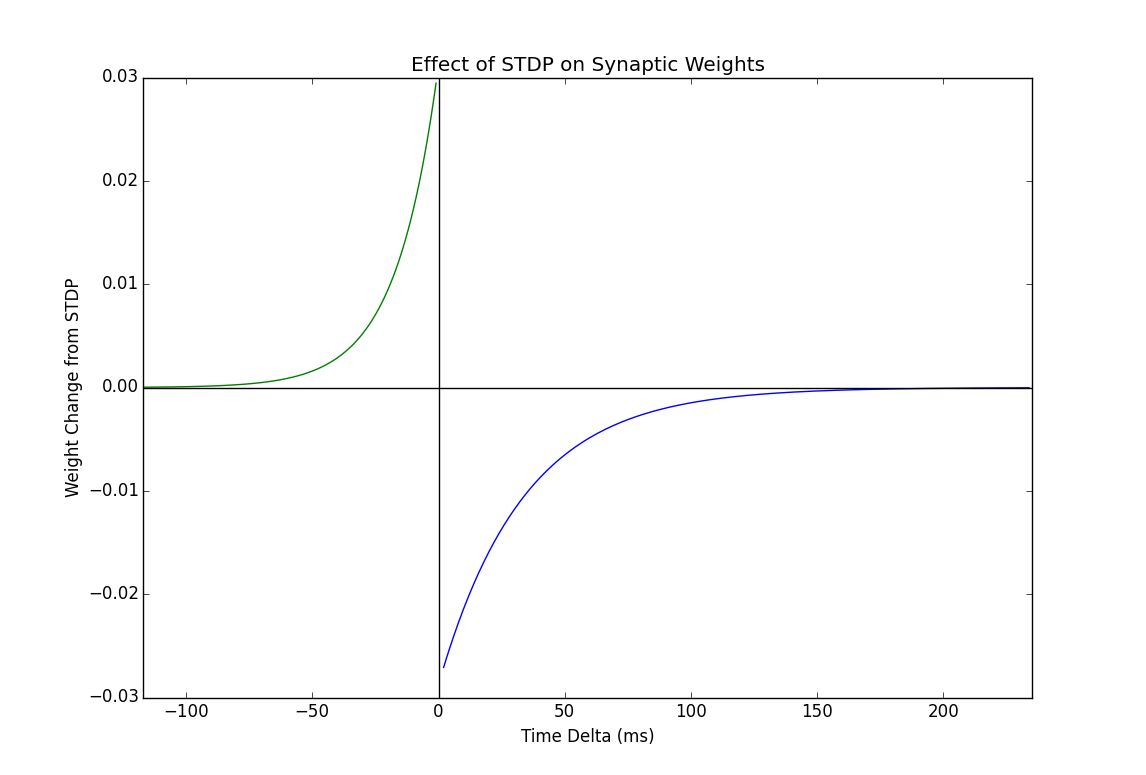
\includegraphics[scale = 0.35]{stdp}
\caption{STDP}
\end{figure}


	Once the pattern recognition neuron becomes selective to the pattern, it continuously reinforces the connections of the afferents that fired slightly before it discharged. Hence with every manifestation of the pattern, the neuron is more likely to fire earlier within it, effectively signalling its beginning. In order to allow for different pattern recognition neurons to become selective to different patterns, we followed Masquelier et al. (2009), connecting a network of pattern recognition neurons to the sample inputs, introducing inhibitory connections amongst the post-synaptic neurons. This allows for a single postsynaptic neuron to become selective to one pattern and to inhibit other postsynaptic neurons from becoming selective to that pattern, thus allowing them to bind to other patterns in the input.\par

Anticipating that the CSTMD1 module would output approximately 500 spike trains, we tuned the pattern recognition neurons from Masquelier et al. to be sensitive to patterns produced by a subset of this number of neurons. As shown in figures [XXX] one pattern recognition neuron becomes sensitive to a recurring pattern produced by 50\% of its afferents, with the synaptic weights to certain afferents involved in the pattern becoming fully potentiated, while the rest are completely depressed. In a 50 second simulation, during the fourth quarter the neuron fires consistently when the pattern manifests itself, with a false-positive and false-negative rate of 0\%.

\begin{figure}[H]
\centering
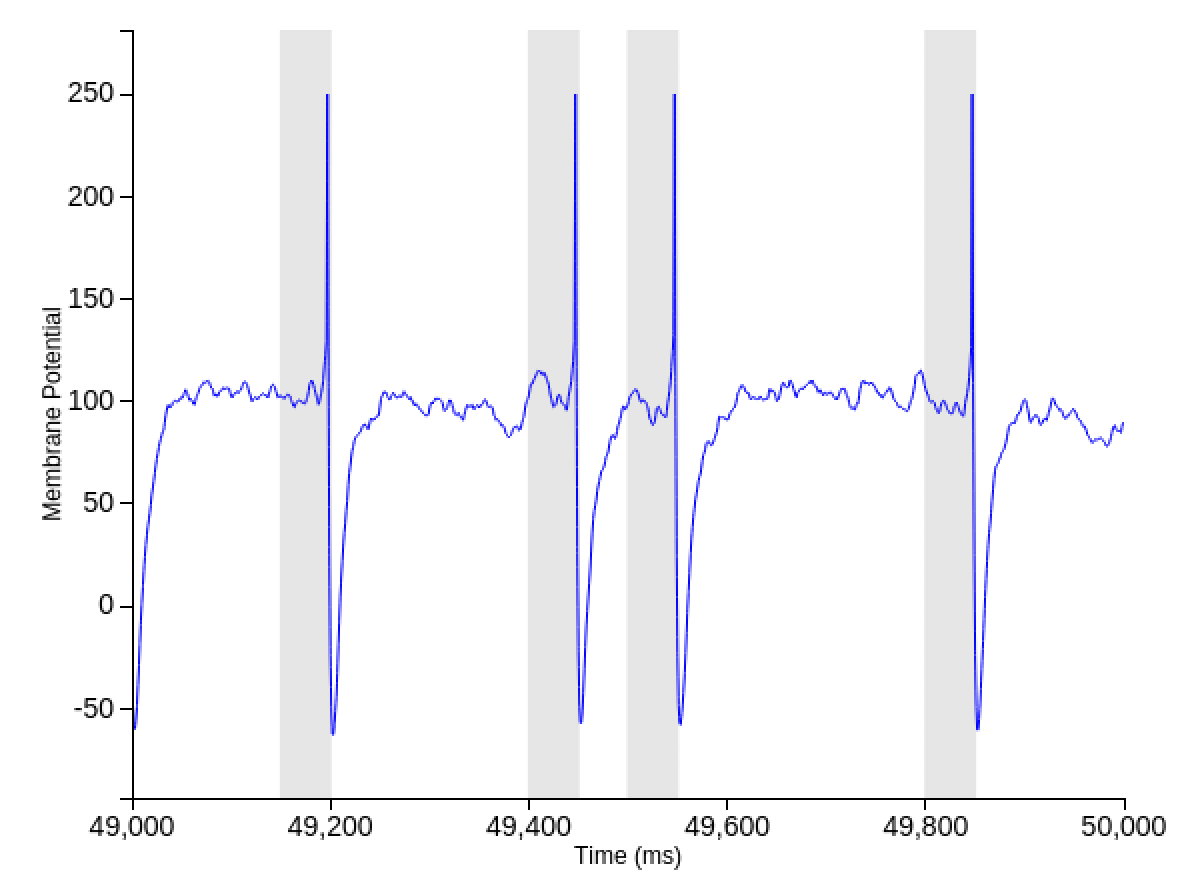
\includegraphics[scale = 0.4]{pr1}
\caption{Neuron fires only when pattern manifests itself. The grey bars indicate when the pattern occurs.}
\end{figure}

\begin{figure}[H]
\centering
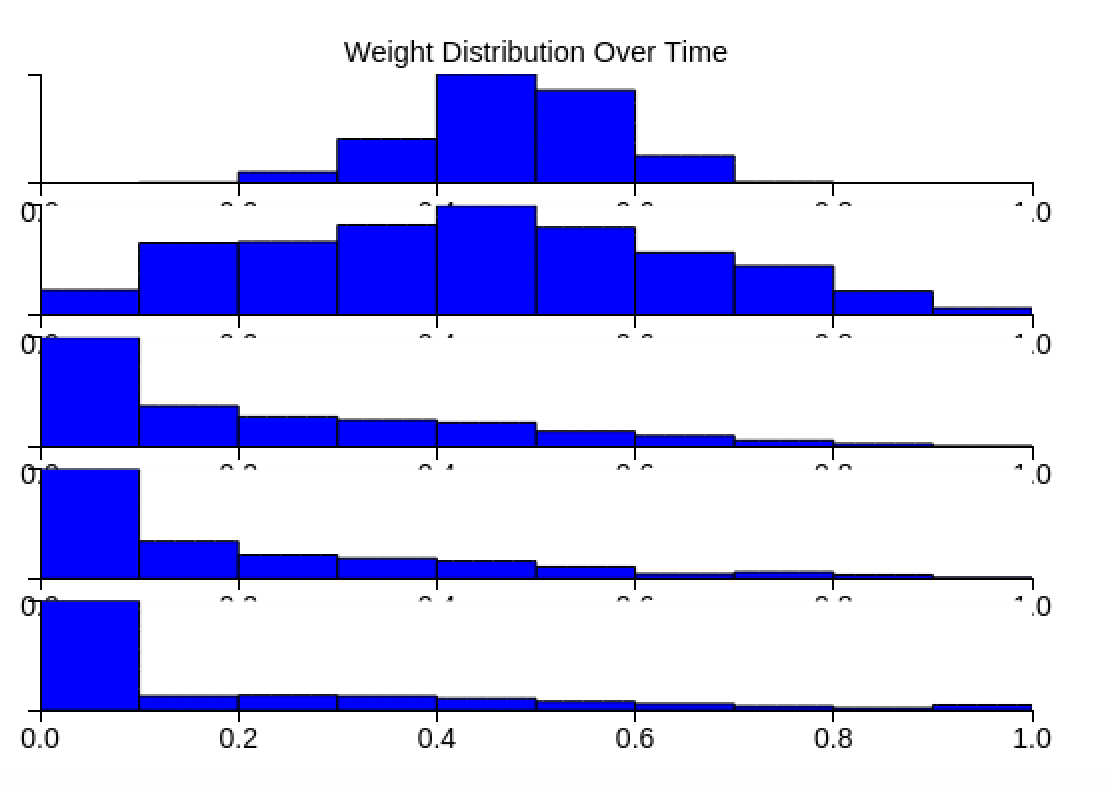
\includegraphics[scale = 0.35]{pr2}
\caption{Distribution of strength of weights for five progressive time slices.}
\end{figure}

\begin{figure}[H]
\centering
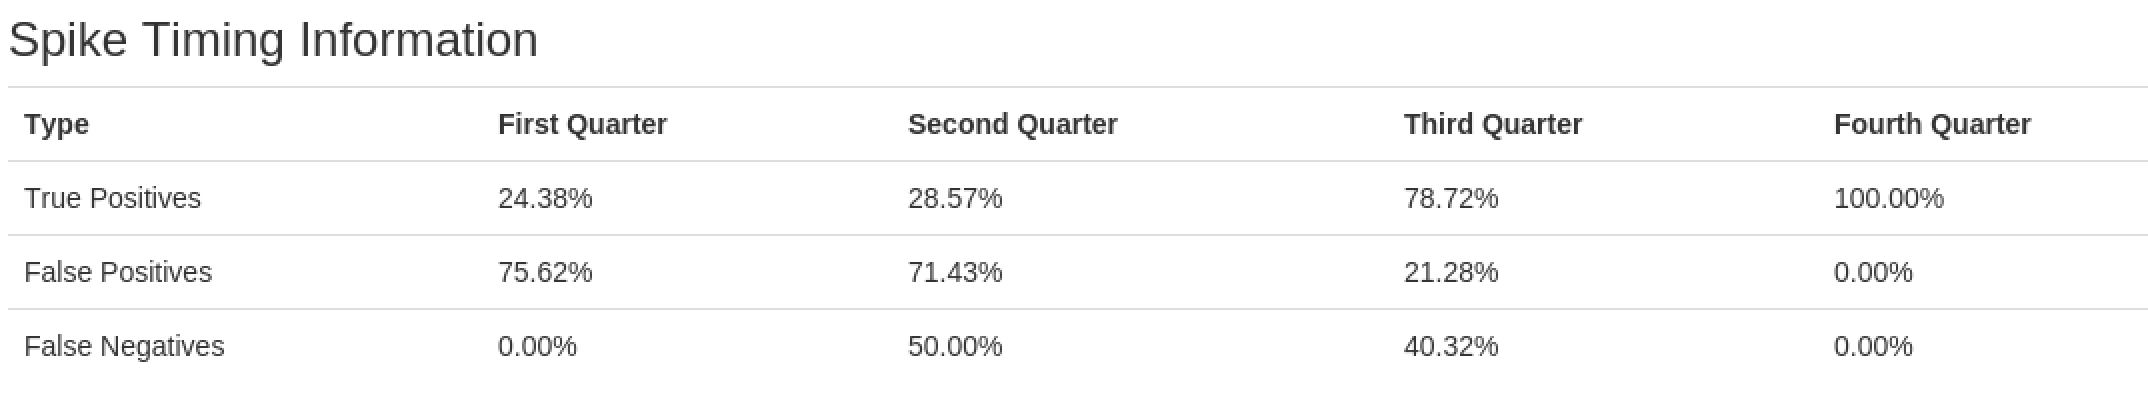
\includegraphics[scale = 0.35]{pr3}
\caption{Rates}
\end{figure}


We produced a similar result with five neurons exposed to three different patterns.

	Once the pattern recognition module was built, we extended it so that the neurons can be easily adapted to recognise input with varying properties such as average firing rate, number of afferents, frequency of pattern appearance, amongst others. This implementation is able to recognise patterns output from our CSTMD1 neurons and is described in section X.X.

\subsection{Action Selection}

The function of this module is to convert the output of the pattern recognition neurons into an action for the dragonfly to take in order for it to pursue insects in its visual field.
The main aspects we needed to consider were:
\begin{enumerate}
	\item The simulation environment of the dragonfly
	\item The embodiment of the dragonfly
	\item The actions available to the dragonfly within its environment
	\item How to convert the output of the pattern recognition neurons into actions
\end{enumerate}
Since the purpose of this project is to provide a tool for studying dragonfly vision rather than prey capture, we decided that having a complicated 3D simulated environment for the dragonfly was unnecessary. Instead, we decided to use the original retina input as a basis for the 'environment' for the dragonfly, and simply add a red circle to the animation input that corresponds to the dragonfly's focal point. The focal point would be moved around within the 2D plane of the visual input by the action selection mechanism and the focal point being overlapping with a target in the visual field would represent the dragonfly having caught the target. The actions available to the dragonfly's focal point would be up, down, left and right within the visual field. Therefore, the output of the action selection module would be a video of the original animation with the position of the dragonfly's focal point superimposed to each frame. An example is shown in Figure 1.

\begin{figure}[H]
\centering
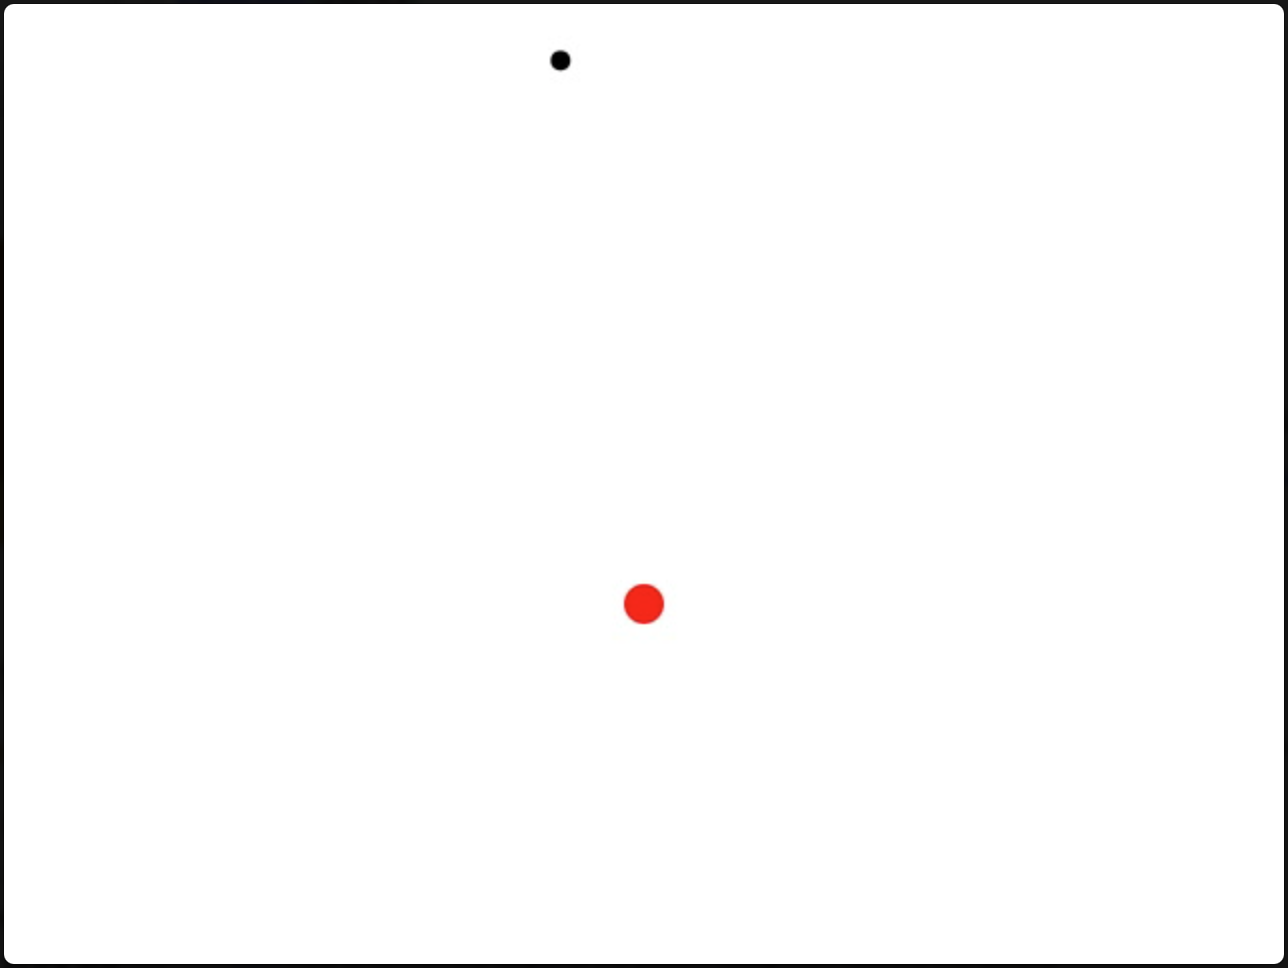
\includegraphics[scale = 0.3]{as_example}
\caption{Simple example of action selection output. The red dot represents the dragonfly focal point and the black dot represents the target.}
\end{figure}

In the original proposal for the project, it was suggested that we use reward-modulated reinforcement learning to train the action selection mechanism. The idea of this is to have a mechanism that can be used to train the dragonfly to choose the actions that maximize its reward, which is administered when it catches a target. 
\newline
\newline
We decided to implement a network of four action selection neurons, each representing one direction of movement (up, down, left and right). These neurons would take as input the spike train output of the pattern recognition neurons, via synapses with all-to-all connections between the two groups of neurons. The weights of the synapses would be initially randomised and the changes in weights would be dynamically governed by spike-timing-dependent plasticity (STDP, the same mechanism as the pattern recognition neurons) but modulated by a reward-modulator, which we label as dopamine but in reality could be another chemical. The way this works is that the change in weights determined by STDP is replaced with an eligibility trace that decays over time and the weights only change when dopamine is present in the system, by multiplying the eligibility trace of each synapse with the level of dopamine present. The dopamine is given a boost whenever the dragonfly focal point is within a certain distance of a target. The conceptual idea is that the synapses that contribute to catching the target are strengthened. The actual model used for the neurons is integrate-and-fire, which is a relatively simplistic but efficient model. The equations that govern the behaviour of the neurons and synapses are shown below: 
\newline
\newline
Integrate-and-fire neurons:
$$\frac{dv}{dt}=\frac{g _{e} (E_{e}-v _{r}) + E_{l} -v}{ \tau_{m}}$$
$$\frac{dg_{e}}{dt}= -\frac{g_{e}}{\tau_{e}}$$
where $v$ is the membrane potential, $g_{e}$ is the synaptic conductance, $E|{e}$ and $E_{l}$ are reverse potentials, $v_{r}$ is the resting potential and $\tau _{m}$ is a time constant.
\newline
Reward-modulated Synapses with STDP:
$$\frac{dw}{dt} = c \cdot Dop$$
$$\frac{dDop}{dt}=-\frac{Dop}{\tau _{Dop}}$$
$$\frac{dc}{dt} = -\frac{c}{\tau _{c}}$$
$$\frac{dApre}{dt}=-\frac{Apre}{\tau_{pre}}$$
$$\frac{dApost}{dt}=-\frac{Apost}{\tau_{post}}$$
where $w$ is the weight of the synapse, $c$ is the eligibility trace, $Dop$ is the level of dopamine, $dApre$ and $dApost$ are variables that govern the STDP and the $\tau$s are time constants.
When the pre-synaptic neuron fires, the following updates are executed:
$$ge = ge + w$$
$$Apre = Apre + Apre _{step}$$
$$c =c+Apost$$
When the post-synaptic neuron fires, the following updates are executed:
$$Apost = Apost + Apost _{step}$$
$$c =c+Apre$$
where $Apre_{step}$ and $Apost_{step}$ are constants.

Finally, at each time step, the distance between dragonfly's focal point (which is initialised to some position at the start) and the nearest target is calculated. If the distance is within a preset distance, a dopamine boost is administered to the system. The movement of the dragonfly is calculated by translating the firing rate of each of the four neurons into the velocity of the focal point in the corresponding direction. The overall velocity and hence distance travelled for the time step was averaged between the four and the dragonfly position updated. 

It is possible to run the action selection part in training mode, where the weights can change, or in fixed mode where you give it trained, fixed weights to simply run a simulation. 

The model was implemented in Python using a neuron simulator package called Brian 2 (CITATION). We used this as it is a flexible simulator and easier to use than NEURON (which was used for the CSTMD), since we are only modelling point neurons in this module, not a multi-compartmental model. 

The output of the action-selection module is twofold:
\begin{enumerate}
\item A video of the original animation with the dragonfly focal point position superimposed to each frame. This way you can see if the dragonfly is 'chasing' the targets or not.
\item A graphical display of the behaviour of variables of the model during the simulation, including weights, firing rates, the dopamine level and a raster plot.
\end{enumerate}
In the web client, the user is able to change the parameters of the model and observe how the resulting dragonfly's behaviour, as well as the behaviour of variables in the model.

\subsection{Web Client}
The web client is designed to be a simple interface through which simulations for each of the modules can be run and automated, both separately and jointly. This graphical user interface interacts with each module's API and provides the functionality needed to save and access the results of every experiment.

In order to maintain consistency with the rest of the project, we decided to use a web framework for Python that could easily connect with each of our modules. The basic requirements were that the client could be easily deployed on a local environment for testing purposes, but also able to serve multiple users concurrently when deployed in production. We chose Bottle \cite{bottle} as it is a lightweight web framework with a built-in HTTP development server that would address the first requirement out-of-the-box. It can also be paired with Nginx \cite{nginx} through uWSGI \cite{uwsgi}. By using Nginx, a high-performance HTTP server on top of uWSGI, a full stack interface between web frameworks and web servers, our web client can be deployed in production, providing load-balanced high-availability.

Given that running our modules' simulations is computationally expensive, it was imperative that the output and results of each run be saved in a persistent store. As shown in figure X, our project consists of five modules connected sequentially, with the output of the each module in the sequence serving as input to the next module. By saving the output of each module during a simulation, we would be able to perform multiple runs of the next module in the sequence without rerunning the previous modules. Additionally, by saving the data generated by each run, the web client can provide a view of the results for analysis by simply querying the database instead of generating them from scratch.

We chose MongoDB, a documented-oriented database, as a data store as it provides a fast, scalable solution that does not require strict design decisions in advance. As we developed our product, MongoDB's dynamic schemas allowed us to modify our objects without having to spend considerable time fixing compatibility issues. Additionally, MongoDB documents follow a JavaScript Object Notation (JSON)-like structure, which mirrors the structure of our Python objects, making it straight forward to understand what fields in our stored documents correspond to what properties of our Python classes.\\
\\
\\
\begin{minipage}[t]{0.5\textwidth}
\centering  
Animation Object as stored in MongoDB
\begin{minted}{python}
  
{
"width": 640,
"height": 480,
"num_frames": 50,
"background_id": "5fde0d",
"description": "Sample.",
"frames_per_second": 5,
"targets":
	[
	{ "color": "rgb(20,97,107)",
	  "velocity": "5",
	  "velocity_vector": [1, 2],
	  "type": 1,
	  "start_pos": [1,2],
	  "frames": 50,
	  "size": 1 },
	  ...
	]
}
\end{minted}
\end{minipage} 
\begin{minipage}[t]{0.5\textwidth}
\centering  
Animation Object constructor in Python
\begin{minted}{python}	
def __init__(self,
  	   width=640,
  	   height=480,    
  	   num_frames=50,
  	   background_id="5fde0d",
  	   description="Sample.",
  	   frames_per_second=5,
  	   targets=[
  	     Target(
	         color="rgb(20,97,107)",
	         velocity=5,
	         velocity_vector=[1,2],
	         type=1,
	         start_pos=[1,2],
	         frames=50,
	         size=1),
	...
	]
):
\end{minted}
\end{minipage}
\\
\\
\\ 
Bottle has a built-in templating engine that enhances HTML5 with a thin layer of Python that can be inserted as both as inline and embedded snippets. These templates also allow the server to pass an object to the view, which can then be accessed using straightforward Python dictionary syntax. As shown in the code snippet below, this makes it easier for create reusable views that dynamically iterate through, access and display relevant content according to the objects made accessible by the server.

\begin{minted}{html}
<!DOCTYPE html>
<html>
% include('head.tpl', title="Pattern Recognition Simulation")
<body>
% include('header.tpl')
...
	<!-- Tab Panes -->
	<div class="tab-content">
	% for i in range(len(simulation['potential_plots'])):
	% p_plot = simulation['potential_plots'][i]
	<div role="tabpanel" class="tab-pane" id="p{{i + 1}}">
		{{!p_plot}}
	</div>
	%end
	</div>
...
% include('footer.tpl')
</body>
</html>
\end{minted}

We also minimised the overhead for our front-end requirements by taking advantage of HTML5 functionalities, such as client-side form validation, video rendering and SVG graphics support. Using jQuery \cite{jquery}, a rich cross-browser JavaScript library, we implemented Asynchronous JavaScript and XML (AJAX) communication between the back-end and the front-end, as well as compatible manipulation of HTML's Document Object Model (DOM) that improves user interaction with the client. Where possible, we converted our graphics from matplotlib to D3.js \cite{d3js}, which provides data visualisation tools for browsers, using the Python API provided by mpld3 \cite{mpld3}. Furthermore, we structured our HTML5 and CSS using Bootstrap \cite{bstrap}, which provides responsive, elegant components for web projects. 


\subsection{Software Engineering Techniques}
The following section describes the framework we used to structure, plan and control the progress of this project.
It includes two main components: Project Management and Collaboration Tools.
\subsubsection{Project Management}
In order to constantly have a solid understanding of the progress of this project and the significance of any issues that arose in each module we used the following techniques.
\paragraph{Scrum}

Given the complexity of our project and its division into clear working stages, we chose to apply the Scrum Methodology of Agile Development as our project management framework.

\paragraph{Sprints}
The project has been divided into seven two-week sprints starting on 4 February 2015. The first five sprints have been designed to complete the minimum and expected goals, with the last two reserved to refine results, prepare the presentation and optionally implement extensions. Sprint Review meetings will be held every other Wednesday in the presence of co-supervisors Zafeirios Fountas and Pedro Mediano, followed directly by the Sprint Planning meeting for the upcoming sprint. Sprints are being managed using online collaboration tool \href{http://trello.com}{Trello} \cite{trello}, with each task given an estimate of one to eight hours and a priority ranging from one (highest) to three (lowest).

\paragraph{Stand-Ups}
Every weekday the team meets for a brief stand up meeting capped at 15 minutes. During this time, the state of the current sprint is assessed, with each team member outlining what he achieved on the previous day and what he will be working on before the next stand-up. Any possible bottlenecks or roadblocks identified during these stand-ups are later addressed by the Team Leader.

\subsubsection{Collaboration Tools}
To ease the internal team communication and ensure that every member is aware of the work conducted by the rest of the team we used the following means.

\paragraph{Communication Channels}
All of our information exchange is conducted using \href{http://slack.com}{Slack} \cite{slack}, a platform for team communication, which provides each member with visibility to all aspects of the project. Relevant information is shared, discussed and classified using Slack's channeled feeds, with a dedicated channel assigned to each sprint.

\paragraph{Version Control}
We are using Git as our version control system, hosting our remote repository on \href{http://gitlab.com}{GitLab} \cite{gitlab}, which integrates with our communication and project management tools. By taking advantage of web hooks, pushes to the repository can trigger automatic code reviews and unit tests, ensuring code integrity and keeping all team members and supervisors up to date with progress.

\subsection{Testing}
The following section describes our testing methodology, implementation as well as the results acquired after the testing was complete.There is also a brief discussion on the challenges faced during testing of this project.
\subsubsection{Methodology}
Our testing strategy has evolved from simple ``on the run manual testing'' to full systematic unit testing of our entire codebase. We followed our project's modular and class-based architecture while designing our testing structure. Each class has a corresponding test class, whose test methods aim to mirror the methods of the class it is testing. However, it is possible that several test methods cover different parts of the same method, or that in turn one test method covers several methods.

Following the white-box testing strategy, each test class is designed by the team members who wrote the original code and who therefore have the best insight regarding the expected behaviour of the original class. Currently we have focused our testing on covering as many branches as possible, each of which is analysed for the different possible behaviours it may have. We are measuring our code coverage by the percentage of statements covered. We are aiming for 90%+ statement coverage.

As we progress with our development we aim to augment our testing strategy to include component, integration and system tests. Component tests will cover end-to-end cases for each of our modules, while integration tests will cover the connections between each of these components. Finally, system tests will cover the complete project, when all modules have been connected between themselves and the web client.

\subsubsection{Implementation}
Given that all of our code is written in Python, we use Python's unittest framework. To measure code coverage we are using Python's coverage library, which allows us to run tests on each file separately and combine results to create comprehensive reports.

\subsubsection{Results - we need to redo tests}
Our current test coverage is 81\%. Detailed results from our latest test run covering all of our modules can be found in Appendix C.

\subsubsection{Challenges}
As expected much of our code has changed when we added additional modules. Accordingly our tests had to be changed. Furthermore since modules are now completed, we have also added tests for code that was not tested before. Our knowledge of testing has significantly improved since the start of the project.

We found it difficult to test the graphical output that our modules produce. While testing it manually is very straightforward, we encountered problems while writing tests to do so systematically. Solution we employed was to store images of the graphics and check the values of specific pixels against the expected ones, which we defined beforehand.

The lines that are missing are for one of the reasons. Either we are missing one of if-else branches that is almost irrelevant to the execution of the module or the person working on that module ran out of time - only created main tests. 
\clearpage
\section{Group Work}

This section describes the division of the total workload among the group members. Flexibility and adaptation were key in the successful division of the tasks. Juan Carlos Farah assumed the position of the team leader due to his previous working experience in technology related projects.

\subsection{Initial Division}
Initially the team was divided into two subgroups, the first to tackle the Target Animation and the CSTMD1 and the second to work on the Pattern Recognition module. The original estimation was that the Target Animation and CSTMD1 would be much easier than the Pattern Recognition, as the CSTMD1 code was largely provided to us by our supervisors. Therefore Christos Kaplanis along with Ioannis Kasidakis were assigned to the CSTMD1 and Target Animation and Juan Carlos Farah, Erik Grabljevec and Panagiotis Almpouras were assigned to the Pattern Recognition group.

\subsection{Reorganising to meet targets}
As mentioned earlier in the report, the CSTMD1 neuron did not behave as expected. With the addition of the ESTMD neuron and the web client, a reorganisation was required to ensure that the project would progress as smoothly as possible. Erik Grablevec was transferred to work along with Christos Kaplanis on the ESTMD module. Ioannis Kasidakis kept working on the CSTMD1 neuron trying to solve the issues that had arisen. Juan Carlos Farah started working on the web client. Initially he created the general structure and later in cooperation with each member he connected the individual modules to the web client and with each other. Panagiotis Almpouras continued working on the pattern recognition module finalising its design and development.

Later on, a new reorganisation was required. Christos Kaplanis  and Erik Grablevec after having completed the ESTMD module, they were respectively assigned to the Action Selection and the Target Animation.

\subsection{Reports and Testing}
With the reports and testing a general strategy was decided early on. Each member would be responsible for providing unit tests for the components he worked on. Similarly, each member should write the part for the report which was most relevant to the part he worked on. The more generic parts of each report were assigned the member(s) that were least busy at the time before the submission.


\clearpage
\section{Final Product}

As our final product, we have succeeded in creating a flexible, cohesive and portable tool for modelling dragonfly vision and target selection. Overall, we succeeded in completing all of the minimum and expected requirements of our specification, but not without a lot of hard work from the group and many challenges along the way. In the figure below we show some screenshots of our web client.

[HOMEPAGE]
[FORMS]
[RESULTS]


From beginning till completion of this project a lot of hard work was put on it. The complex nature of 
the field of neuroscience as a whole significantly increased the overall level of difficulty of the 
project. Our goal was not just to replicate the neural processes occurring when the dragonfly preys 
but to create a tool that models them in the most realistic way possible and that provides helpful 
metrics for the analysis of those processes.

For most parts we accurately estimated the level of difficulty so that we can properly allocate 
resources on. Some however proved more challenging than we originally expected. This section 
summarises the goals that we met, the targets that we could only partially complete, the reasons
why we could not fully address some of the issues that arose during the project as well as further
development that could prove fruitful in the future.

\subsection{Goals Met}

As can be seen in the Specification section of this report we managed to fully complete most of the 
targets that we set. In fact, we managed to complete all the targets set not only as minimum 
requirements (Stage 1) but also for the expected implementation (Stage 2). More specifically, we 
managed to:

\begin{enumerate}

 \item{Create an animation tool that allows the generation of input for visual processing. (Minimum 
Requirement)}

\item{Build a model for the ESTMD neuron present between the retina and the actual CSTMD1 
neurons of a real dragonfly. The function of this neuron is, given visual input, to isolate small targets 
from a potentially noisy background. (Minimum Requirement)}  

\item{Build a layer of pattern recognition neurons that can be trained in an unsupervised manner to 
identify spike patterns within a noisy background. (Minimum Requirement)}

\item{Integrate the visual processing and pattern recognition system to detect patterns within the
CSTMD1 output and add a simple action selection mechanism. (Minimum Requirement)}

\item{Develop a web client to provide an interface and key metrics for each module and for the 
system as a whole.  (Expected Implementation)}

\item{Create an animation for the dragonfly agent to visualise the results of a simulation. (Expected 
Implementation)}

\item{Enhance the action selection mechanism to control the agent within the environment 
(Expected Implementation)}

\item{Improve the usability and features of the web client (Possible Exentions)}

\end{enumerate}

\subsection{Target Animation}
\begin{figure}[h]
\centering
\begin{minipage}{0.2\textwidth}
\fbox{
\includegraphics[scale = 0.14]{scr0}}
\end{minipage}
\begin{minipage}{0.2\textwidth}
\fbox{
\includegraphics[scale = 0.14]{scr3}}
\end{minipage}
\begin{minipage}{0.2\textwidth}
\fbox{
\includegraphics[scale = 0.14]{scr6}}
\end{minipage}
\begin{minipage}{0.2\textwidth}
\fbox{
\includegraphics[scale = 0.14]{scr9}}
\end{minipage}
\caption{Simple example of action selection output. The red dot represents the dragonfly focal point and the black dot represents the target.}
\label{target_animation_example}
\end{figure}
\subsection{Partially completed tasks}

The task that proved to be the most challenging aspect of the project was the development of the 
CSTMD1 neuron. It is observed that the CSTMD1 neuron when provided with multiple stimuli, it spikes 
depending only on one of them thus providing a selection mechanism \cite{?}. In the beginning of 
the project we were provided with third party code that replicated that process but was tested only 
for a specific type of input. With the visual input that was key to our project however the CSTMD1 
neuron did not show the expected behaviour and it failed to provide a robust selection mechanism. 
Despite our constant efforts to make it work, the time constraints of this project along with the high 
complexity of the other modules made it infeasible to fully meet this target. Therefore the target:\\

\noindent

Achieve CSTMD1 target selection through experimentation with various parameters and connections 
with the ESTMD neuron (Possible Extensions)
was only partially completed.

\subsection{Non-implemented tasks}

Of all the goals that were set there was only one we did not get the chance to work on:

\noindent
Implement the agent in a quadcopter drone (Possible Extensions).
The idea behind this goal was to integrate the completed agent to an actual quadcopter with 
embedded cameras that would allow it to react in real time to stimuli. That however would require
very fast completion of the whole system or extended period of time to work on this project. What is 
more, the required processing of the visual input within each simulation is so computationally 
expensive that made it impossible to implement a real time system with the existing hardware. 
Therefore this goal could not be met.

\subsection{Future Development}
Our project's modular architecture and design allows for future development on each of the components to be feasible both by the members of our team as well as the community. We will release our source code via a public repository and welcome contributions as we continue to improve our tool. Given our use of Git as a source version control system, users will be able to easily clone and fork the repository for their own deployments, as well as submit pull requests to contribute to the development of the original tool. We have also made a public-facing website available at (WEBSITE) so that potential users or contributors can easily test the web client.

Specific areas where our system can be potentially improved include the following:

\begin{enumerate}
\item Neuron Models Adjustable
\item Custom Modules
\item Improve Data Visualisation in the Web Client
\item Improve usability of the web client (multiple users)
\item Implement 3D simulation for target animation and action selection
\item Option to export code for testing in a quadcopter drone
\end{enumerate}

\subsection{Project Evaluation}

Given the positive results that we achieved with the current implementation of our initial specifications,
we are confident that this project has been a success. As a team, it was for us an introduction to the field of
computational neuroscience and even though we were faced with a steep learning curve, we are all satisfied
with the skills we have acquired in the process. We are also encouraged by the fact that we were able to implement
a wide variety of technologies. This breadth has exposed us to the advantages, limitations and uses of various tools,
some of which can be valuable assets for future pursuits in an extensive range of fields. The fact that we were able
to familiarise ourselves with these and integrate them into a system that could be further developed in the
future is an extremely gratifying experience.

We also recognise that teamwork is an important aspect of software engineering and this endeavour has
introduced us to an array of useful development techniques that allowed us to properly cooperate in a flexible
and efficient way. Finally, the contributions and insights from our supervisors were paramount to the success of
this project and we have acquired invaluable insights from this collaboration.







\clearpage

\bibliography{final_report}{}
\bibliographystyle{plain}
\clearpage
\appendix
\section{Logbook}

\clearpage
\section{Minutes of Group Meetings}
\textbf{Logged by: Panagiotis Almpouras}
\subsubsection*{This is a summary of the meeting minutes recorded throughout the project.}
\maketitle
\section*{16 January 2015}
\subsection*{Attendance}
\begin{compactenum}
\item Juan Carlos Farah (JCF)
\item Christos Kaplanis (CK)
\item Erik Grabljevec (EG)
\item Panagiotis Almpouras (PA)
\item Ioannis Kasidakis (IK)
\item Zafeirios Fountas (ZF)
\item Pedro Martínez Mediano(PMM)
\end{compactenum}

\subsection*{Summary}
This meeting was mainly focused on discussing the way the group would tackle administrative tasks. The decision about the split of the groups was finalised and initial tasks (mainly background reading) was assigned to the two groups. The members were split in a group of three (JCF, EG, PA) that would focus on the pattern recognition and a group of two (CK, IK) that would focus on the action selection.

\maketitle
\section*{21 January 2015}
\subsection*{Attendance}
\begin{compactenum}
\item Juan Carlos Farah (JCF)
\item Christos Kaplanis (CK)
\item Erik Grabljevec (EG)
\item Panagiotis Almpouras (PA)
\item Ioannis Kasidakis (IK)
\item Zafeirios Fountas (ZF)
\item Pedro Martínez Mediano(PMM)
\end{compactenum}

\subsection*{Summary}
This meeting was mainly focused on discussing questions we had after reading all the relevant papers as well as what should be the next steps. A joint meeting took place after which, separate group meetings were conducted with each relevant supervisor to discuss in more detail about the specifics of the upcoming tasks.

\maketitle
\section*{28 January 2015}
\subsection*{Attendance}
\begin{compactenum}
\item Juan Carlos Farah (JCF)
\item Christos Kaplanis (CK)
\item Erik Grabljevec (EG)
\item Panagiotis Almpouras (PA)
\item Ioannis Kasidakis (IK)
\item Zafeirios Fountas (ZF)
\item Pedro Martínez Mediano(PMM)
\end{compactenum}

\subsection*{Summary}
This meeting was mainly focused on the progress of the two groups so far. Most tasks (regarding replicating work that has been done by researchers so that members get comfortable with the concepts and methods) were on track and progressing as expected. A decision was made on the general structure of the first report (due on 06/02/2015) and each member was assigned a part of the report that they would have to prepare before the next meeting.

\maketitle
\section*{04 February 2015}
\subsection*{Attendance}
\begin{compactenum}
\item Juan Carlos Farah (JCF)
\item Christos Kaplanis (CK)
\item Erik Grabljevec (EG)
\item Panagiotis Almpouras (PA)
\item Ioannis Kasidakis (IK)
\item Zafeirios Fountas (ZF)
\item Pedro Martínez Mediano(PMM)
\end{compactenum}

\subsection*{Summary}
This meeting was mainly focused on the first report. With the input of the supervisors and the slides provided by the course instructor Dr. Fidelis Perkonigg the final structure of the report was decided and a soft deadline was set for completion, to allow for a few last amendments before the actual submission on the 06/02/2015.

\maketitle
\section*{11 February 2015}
\subsection*{Attendance}
\begin{compactenum}
\item Juan Carlos Farah (JCF)
\item Christos Kaplanis (CK)
\item Erik Grabljevec (EG)
\item Panagiotis Almpouras (PA)
\item Ioannis Kasidakis (IK)
\item Zafeirios Fountas (ZF)
\item Pedro Martínez Mediano(PMM)
\end{compactenum}

\subsection*{Summary}
This meeting was mainly focused on the progress and issues of each group. The pattern recognition group (JC, EG, PA) had no issues to report and made progress according to plan. The action selection group (CK, IK) upon completion of the initial tasks realised they need an extra component to act as an intermediate between the stimuli input and the action selection neurons. The main issue was the isolation of the small moving targets from much larger objects that may be moving in the background. The action selection group set a goal for next week to identify the most feasible solution by conducting deep background research on the topic.

\maketitle
\section*{18 February 2015}
\subsection*{Attendance}
\begin{compactenum}
\item Juan Carlos Farah (JCF)
\item Christos Kaplanis (CK)
\item Erik Grabljevec (EG)
\item Panagiotis Almpouras (PA)
\item Ioannis Kasidakis (IK)
\item Zafeirios Fountas (ZF)
\item Pedro Martínez Mediano(PMM)
\end{compactenum}

\subsection*{Summary}
This meeting was mainly focused on the progress and issues of each group. The pattern recognition group (JC, EG, PA) had no issues to report and made progress according to plan. The pattern recognition was providing accurate results and was modularised so that it could run independently given a proper input.
\\ The action selection group (CK, IK) upon completion of the initial tasks realised they need an extra component to act as an intermediate between the stimuli input and the action selection neurons. The main issue was the isolation of the small moving targets from much larger objects that may be moving in the background. The action selection group set a goal for next week to identify the most feasible solution by conducting deep background research on the topic.

\maketitle
\section*{25 February 2015}
\subsection*{Attendance}
\begin{compactenum}
\item Juan Carlos Farah (JCF)
\item Christos Kaplanis (CK)
\item Erik Grabljevec (EG)
\item Panagiotis Almpouras (PA)
\item Ioannis Kasidakis (IK)
\item Zafeirios Fountas (ZF)
\item Pedro Martínez Mediano(PMM)
\end{compactenum}

\subsection*{Summary}
This meeting was mainly focused on the action selection mechanism. The action selection group managed to identify a viable solution to the issues mentioned in last week's meeting. An intermediate mechanism should be constructed to approximate the function of the ESTMD neuron. The function of the mechanism would be to pre-process the visual input to isolate small targets. Since the pattern recognition group had almost completed its task one member (EG) was transferred to the action selection group to assist with the development of  ESTMD . A web client was also deemed as a good addition to the project to provide a user friendly interface that connects all the modules together but also allows for independent use of each. The pattern recognition group was further split. One member would focus on the web client (JCF) and the other (PA) would continue working on the pattern recognition mainly creating unit tests to ensure that future changes would not create unspotted issues that affect the robustness and accuracy of the module.

\maketitle
\section*{4 March 2015}
\subsection*{Attendance}
\begin{compactenum}
\item Juan Carlos Farah (JCF)
\item Christos Kaplanis (CK)
\item Erik Grabljevec (EG)
\item Panagiotis Almpouras (PA)
\item Ioannis Kasidakis (IK)
\item Zafeirios Fountas (ZF)
\item Pedro Martínez Mediano(PMM)
\end{compactenum}

\subsection*{Summary}
This meeting was mainly focused on the web client and the ESTMD neuron. A skeleton version of the web client was created by (JCF) and the next step would be to connect the completed pattern recognition module to the web client. Progress was reported on the ESTMD, however the intermediate mechanism revealed some unspotted issues with the CSTMD neuron that is responsible for selecting a single target if multiple stimuli are provided. The action selection group was divided into two sub-groups. Two members (CK, EG) would continue working on the ESTMD and the third member (IK) would focus on the CSTMD to analyse the erroneous behaviour and identify potential solutions. The structure of the second report (due on 13/03/2015) was also discussed.

\maketitle
\section*{11 March 2015}
\subsection*{Attendance}
\begin{compactenum}
\item Juan Carlos Farah (JCF)
\item Christos Kaplanis (CK)
\item Erik Grabljevec (EG)
\item Panagiotis Almpouras (PA)
\item Ioannis Kasidakis (IK)
\item Zafeirios Fountas (ZF)
\item Pedro Martínez Mediano(PMM)
\end{compactenum}

\subsection*{Summary}
This meeting was mainly focused on the second report. With the input of the supervisors and the slides provided by the course instructor Dr. Fidelis Perkonigg the final structure of the report was decided and a soft deadline was set for completion, to allow for a few last amendments before the actual submission on the 13/03/2015.

\maketitle
\section*{18 March 2015}
\subsection*{Attendance}
\begin{compactenum}
\item Juan Carlos Farah (JCF)
\item Christos Kaplanis (CK)
\item Erik Grabljevec (EG)
\item Panagiotis Almpouras (PA)
\item Ioannis Kasidakis (IK)
\item Zafeirios Fountas (ZF)
\item Pedro Martínez Mediano(PMM)
\end{compactenum}

\subsection*{Summary}
This meeting was mainly focused on the web client and the ESTMD neuron. The action selection module was successfully connected to the web client and some prefixed simulations could be run online. Next step would be to add as many functionalities as possible to the web client before the completion and connection of the other modules. Progress was reported on the ESTMD development (CK,EG). No progress was reported on the CSTMD neuron (IK) but a lot of possible ways to address the issue were discussed and would be looked into before the next meeting.

\maketitle
\section*{25 March 2015}
\subsubsection*{No meeting was held this week due to examinations.}

\maketitle
\section*{1 April 2015}
\subsection*{Attendance}
\begin{compactenum}
\item Juan Carlos Farah (JCF)
\item Christos Kaplanis (CK)
\item Erik Grabljevec (EG)
\item Panagiotis Almpouras (PA)
\item Ioannis Kasidakis (IK)
\item Zafeirios Fountas (ZF)
\item Pedro Martínez Mediano(PMM)
\end{compactenum}

\subsection*{Summary}
This meeting was mainly focused on planning the group project activities to take place during the exam preparation period. Members mutually agreed to focus on exams and work on the group project one day a week for the following weeks. Slower but steady progress was expected.  The CSTMD neuron proving much more challenging than originally expected was the only section for which an accurate estimate of the completion date could not be made. For that reason the simpler but similar mechanism of the point neurons was decided to be the last resource in case the CSTMD could not function properly.

\maketitle
\section*{8 April 2015}
\subsubsection*{No meeting was held this week due to Easter holiday.}

\maketitle
\section*{15 April 2015}
\subsection*{Attendance}
\begin{compactenum}
\item Juan Carlos Farah (JCF)
\item Christos Kaplanis (CK)
\item Erik Grabljevec (EG)
\item Panagiotis Almpouras (PA)
\item Ioannis Kasidakis (IK)
\item Zafeirios Fountas (ZF)
\item Pedro Martínez Mediano(PMM)
\end{compactenum}

\subsection*{Summary}
This meeting was mainly focused on discussing the progress of the development of the several modules. The web client was progressing as expected and as soon as each module was completed it would get connected to the web client. The ESTMD was progressing as expected and completed. The CSTMD still could not progress. The target animation along with the re-enforcement learning mechanism were the next things to be tackled. The target animation was assigned to (PA) and (EG), the re-enforcement learning was assigned to (CK). (JCF) would continue working on the web client and (IK) on the CSTMD and the point neurons.

\maketitle
\section*{22 April 2015}
\subsection*{Attendance}
\begin{compactenum}
\item Juan Carlos Farah (JCF)
\item Christos Kaplanis (CK)
\item Erik Grabljevec (EG)
\item Panagiotis Almpouras (PA)
\item Ioannis Kasidakis (IK)
\item Zafeirios Fountas (ZF)
\item Pedro Martínez Mediano(PMM)
\end{compactenum}

\subsection*{Summary}
This meeting was mainly focused on discussing the progress of the development of the several modules. All modules apart from CSTMD were progressing as expected. The CSTMD showed some progress. All members mutually agreed not to work on the group project during the following two weeks as the final exams where taking place during that period.

\maketitle
\section*{29 April 2015}
\subsubsection*{No meeting was held this week due to examinations.}

\maketitle
\section*{6 May 2015}
\subsubsection*{No meeting was held this week due to examinations.}

\maketitle
\section*{8 March 2015}
\subsection*{Attendance}
\begin{compactenum}
\item Juan Carlos Farah (JCF)
\item Christos Kaplanis (CK)
\item Erik Grabljevec (EG)
\item Panagiotis Almpouras (PA)
\item Ioannis Kasidakis (IK)
\item Zafeirios Fountas (ZF)
\item Pedro Martínez Mediano(PMM)
\end{compactenum}

\subsection*{Summary}
This meeting was mainly focused on creating a schedule for the activities to take place during the last week before the submission. (JCF) would work with each member to make the final connection of all the modules to the web client. (IK) would finish the CSTMD neuron asap to test its behaviour. (PA) would start working on the report, creating the main structure and writing any part that can be written without the input of another member (mainly Introduction,  Specification, Group Work, Appendix). A soft deadline was set for completion of the report on the 12/04/2015, to allow for a few last amendments before the actual submission on the 15/04/2015.

\maketitle
\section*{13 May 2015}
\subsection*{Attendance}
\begin{compactenum}
\item Juan Carlos Farah (JCF)
\item Christos Kaplanis (CK)
\item Erik Grabljevec (EG)
\item Panagiotis Almpouras (PA)
\item Ioannis Kasidakis (IK)
\item Zafeirios Fountas (ZF)
\item Pedro Martínez Mediano(PMM)
\end{compactenum}

\subsection*{Summary}
This meeting was mainly focused on the final report. With the input of the supervisors and the materials provided by the course instructor Dr. Fidelis Perkonigg the contents of the report were finalised. A brief discussion on the presentation took place. The presentation would be prepared after the submission of the final report on the 15/04/2015 as the date of the presentation was set to be the 19/05/2015.



\clearpage
\section{Detailed Work Breakdown}

\begin{table}[h]
\centering
\begin{tabular}{|l|l|l|}
\cline{1-3}
Member& Task&  Time  \\ \cline{1-3}
 Juan Carlos Farah&  Pattern Recognition Module&  6.5 weeks  \\ \cline{1-3}
&  Web Client&  4.5 weeks  \\ \cline{1-3}
& Testing& 0.5 weeks \\ \cline{1-3}
&  First Report&  0.5 week  \\ \cline{1-3}
&  Second Report&  0.5 week  \\ \cline{1-3}
&  Final Report& 1.0 week   \\ \cline{1-3}
&  &    \\ \cline{1-3}
Panagiotis Almpouras&  Pattern Recognition Module& 8.0 weeks  \\ \cline{1-3}
&  Testing&  2.0 weeks  \\ \cline{1-3}
&  First Report&  0.5 week  \\ \cline{1-3}
&  Second Report&  0.5 week  \\ \cline{1-3}
&  Final Report&  1.5 weeks  \\ \cline{1-3}
&  &    \\ \cline{1-3}
 Christos Kaplanis&  ESTMD Module&  5.5 weeks  \\ \cline{1-3}
&  CSTMD module& 2 weeks    \\ \cline{1-3}
&  Action Selection Module&  3.5 weeks  \\ \cline{1-3}
& Testing& 0.5 weeks \\ \cline{1-3}
&  First Report&  0.5 week  \\ \cline{1-3}
&  Second Report&  0.5 week  \\ \cline{1-3}
&  Final Report&  1.0 week  \\ \cline{1-3}
&  &   \\ \cline{1-3}
Erik Grabljevec&  Pattern Recognition Module&  3.0 weeks  \\ \cline{1-3}
&  ESTMD Module&  4.0 weeks  \\ \cline{1-3}
&  Target Animation&  3.5 weeks  \\ \cline{1-3}
& Testing& 0.5 weeks \\ \cline{1-3}
&  First Report& 0.5 week  \\ \cline{1-3}
&  Second Report&  0.5 week  \\ \cline{1-3}
&  Final Report&  1.0 week  \\ \cline{1-3}
&  &   \\ \cline{1-3}
Ioannis Kasidakis& CSTMD Module& 9 weeks  \\ \cline{1-3}
&  Web Client & 3.5 weeks    \\ \cline{1-3}
& Testing& 0.5 weeks \\ \cline{1-3}
&  First Report& 0.5 week     \\ \cline{1-3}
&  Second Report& 0.5 week   \\ \cline{1-3}
&  Final Report& 1.0 week   \\ \cline{1-3}

\end{tabular}
\end{table}


\end{document}

